% Copyright (c) 2014,2016 Casper Ti. Vector
% Public domain.
\chapter{Observation of $Z_{cs}$ states in $\Bp\to\jpsi\phi\Kp$ decay}
%\chapter{Dataset, Reconstruction and Selections}
\label{chap:Zcs_study}

%%\section{Previous study and $Z_{cs}$ prediction}
\section{Study motivation}

Since the discovery of the $X(3872)$ state by the \belle experiment in 2003\supercite{PhysRevLett.91.262001}, 
more than twenty non-conventional hadrons that contain $\ccbar$ or $\bbbar$ quarks have been found and studied\supercite{PDG2020}. 
In contrast to the neutral states, 
charged states like $Z_c(3900)^+$\supercite{PhysRevLett.110.252001,PhysRevLett.110.252002} and $Z_c(4430)^+$\supercite{Choi:2007wga, Chilikin:2013tch, LHCb-PAPER-2014-014} provide evidence for tetraquark exotic states, 
because light quarks are required to account for the non-zero electric charge in addition to the heavy quarkonium.
\footnote{Charge conjugation is implied throughout this thesis.} 
Previously, 
only the \uquark or \dquark quarks were observed to constitute the light quark content of such charged exotic states, 
even though the existence of a $Z_{cs}$ state as a strangeness-flavour partner of the $Z^+_c(3900)$ state 
has been predicted\supercite{Voloshin:2019ilw,Dias:2013qga,Chen:2013wca,Ferretti:2020ewe,Lee:2008uy}.
%As mentioned in Section.~\ref{subsubsec:01_Zcs_observation},
Therefore,
it is an important research topic to search the hiddren charm tetraquark with strangeness in hadron spectroscopy field,
the property of this type of states can help test different theoritical predictions to nonstandard hadron states. 
%Besides, the measured widths of $X(4140)$ among different experiments ^ 

\subsection{Previous studies}
%Among all known decays of $b-$hadrons, 
%$\Bp\to\jpsi\phi K^+$ are unique, 
%since conventional hadron contributions from kaon excitations (hereafter denoted as $K^{*+}\to\phi K^+$) are broad, 
%and visible mass structures on the Dalitz plot are dominated by a number of relatively narrow $X\to\jpsi\phi$ states, 
%which are candidates for tetraquarks with hidden-charm and hidden-strangeness. 
%Contributions from these exotic hadron components approach half of the entire rate in this decay channel.
%The first evidence for the $\jpsi\phi$ state was observed by CDF~\supercite{Aaltonen:2009tz}. 
%A very narrow ($\Gamma=15.3_{-\phantom{1}6.1}^{+10.4}\pm2.5$\mev), 
%near-threshold ($M=4143.4\pm3.0\pm0.6$\mev) 
%$X(4140)$ state was claimed.
%\footnote{The recent PDG naming convention calls this state $\chi_{c1}(4140)$. 
%However, 
%generic $X$ label is used for $\jpsi\phi$ states, 
%which is independent of their $J^P$ assignments.} 
%Such narrow structure was not confirmed by the Belle~\supercite{ChengPing:2009vu}, Babar~\supercite{Lees:2014lra}, 
%and early low-statistics LHCb~\supercite{LHCb-PAPER-2011-033} data. 
%However, 
%the near-threshold state was observed by the CMS collaboration~\supercite{Chatrchyan:2013dma}. 
%There was also an evidence for it from the D0 experiment~\supercite{Abazov:2013xda}. 
%An evidence for a second structure, $X(4274)$, in the CDF and CMS data was observed. 
%The $\jpsi\phi$ mass distribution among $2480\pm160$ $\Bp\to\jpsi\phi K^+$ events detected by CMS is shown in Figure.~\ref{fig:newfig3}, 
%which was obtained after the subtraction of a very large combinatorial background.  
%
%\begin{figure}[b]
%  \begin{center}
%  \vspace{-0.3cm}
%   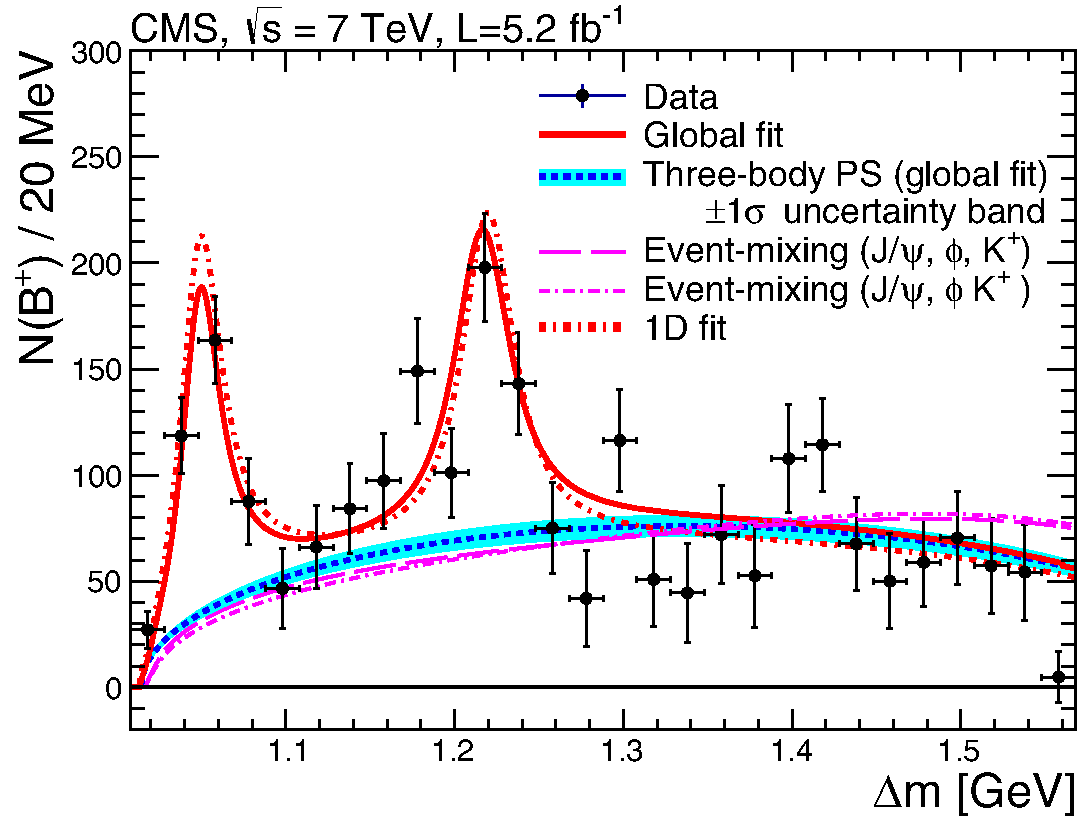
\includegraphics[width=0.4\textwidth]{Figures/01_Introduction/Physics/from_Zcs/newFig3.pdf}
%     \vskip -0.4cm
%    \caption{\small
%The number of  $\Bp\to\jpsi\phi K^+$  candidates as a function
%of $\Delta m = m(\mu^+\mu^-\Kp\Km)-m(\mu^+\mu^-)$.
%    }
%    \label{fig:newfig3}
%  \end{center}
%\end{figure}

%LHCb~\supercite{LHCb-PAPER-2016-018,LHCb-PAPER-2016-019} performed the first amplitude analysis of $\Bp\to\jpsi \phi K^+$ decays, 
%investigating the $\jpsi \phi$ structures in Run 1 data. 
%The number of $\Bp\to\jpsi \phi K^+$ signal events was $4289\pm141$ with a background fraction of $23\%$. 
%The data could be described including seven $K^{*+}\to\phi K^+$ resonances, 
%determined by the fit and consistent with either known or predicted states, 
%four $X\to\jpsi\phi$ structures, and non-resonant $\phi K^+$ and $\jpsi \phi$ contributions. 
%The mass projections of $\phi K^+$ and $\jpsi \phi$ combinations are shown in Figure.~\ref{fig:defmasses}. 
%Table~\ref{tab:run1} shows the results, including the determined masses, widths, fit fractions and spin-parity assignments. 
%The four $X$ structures and a non-resonant $\jpsi \phi$ contribution all had significance above 5$\sigma$. 
%The existence of $\Xtwo$ was established. 
%The quantum numbers of $\Xone$ and $\Xtwo$ states were identified as $1^{++}$ at  $>5\sigma$ significance, 
%while the $\Xthree$ and $\Xfour$ states as $0^{++}$ at $>4\sigma$. Notably, the $\Xone$ width was substantially larger than previously determined. 
%
%\begin{figure}[hbtp]  
%  \begin{center}
%    \includegraphics[width=0.5\textwidth]{Figures/01_Introduction/Physics/from_Zcs/newbase_PhiKh.pdf}%
%    \includegraphics[width=0.5\textwidth]{Figures/01_Introduction/Physics/from_Zcs/newbase_JpsiPhih.pdf} 
%  \end{center}
%\caption{
%    Distributions of $\phi K^+$ (left) and $\jpsi\phi$ (right)
%    invariant masses for the $\Bp\to\jpsi \phi K^+$ candidates (black data points) 
%    compared with the results of the default amplitude fit
%    to the Run 1 data \supercite{LHCb-PAPER-2016-018}.}
%  \label{fig:defmasses}
%\end{figure} 


\begin{table}[h]
\centering
\caption{Results from previous publication based on Run 1 data at \lhcb\supercite{LHCb-PAPER-2016-018}.}\label{tab:run1}

\begin{tabular}{cccccc}
\hline
\multicolumn{2}{c}{Contribution} &Significance & \multicolumn{3}{c}{Fit results} \\
                &                                  &            & $M_0$ [MeV]   & $\Gamma_0$ [MeV]      & FF\% \\
\hline \hline
&      All K($1^+$)   & 8.0$\sigma$       &      &      &  $42\pm 8^{+5}_{-9}$  \\
   &      ${\rm NR}_{\phi K}$  &       &      &      &  $16\pm 13^{+35}_{-6}$  \\
$\nslj{2}{1}{P}{1}$   &    K($1^+$)   & 7.6$\sigma$       &  $1793\pm 59^{+153}_{-101} $   &   $365\pm 157^{+138}_{-215} $   &  $12\pm 10^{+17}_{-6}$ \\
$\nslj{2}{3}{P}{1}$     &    $K^{\prime}$($1^+$)   & 1.9$\sigma$       &  $1968\pm 65^{+70}_{-172} $   &   $396\pm 170^{+174}_{-178} $   &  $23\pm 20^{+31}_{-29}$   \\
\hline
   &       All K($2^-$)   & 5.6$\sigma$       &      &      &  $11\pm 3^{+2}_{-5}$  \\
$\nslj{1}{1}{D}{2}$   &  $K_2 (1770)$     & 5.0$\sigma$       &  $1777\pm 35^{+122}_{-77} $   &   $217\pm 116^{+221}_{-154} $   & \\
$\nslj{1}{3}{D}{2}$ &  $K_2(1820)$   & 3.0$\sigma$       &  $1853\pm 27^{+18}_{-35} $   &   $167\pm 58^{+83}_{-72} $   &   \\       
\hline    
& $K(1^-)$ \\
$\nslj{1}{3}{D}{1}$  &  $K^*(1680)$  &    8.5$\sigma$       &  $1722\pm 20^{+33}_{-109} $   &   $354\pm 75^{+140}_{-181} $   & $6.7 \pm 1.9^{+3.2}_{-3.9}$ \\  
\hline 
& $K(2^+)$\\

$\nslj{2}{3}{P}{2}$  &  $K^*_2(1980)$   & 5.4$\sigma$       &  $2073\pm 94^{+245}_{-240} $   &   $678\pm 311^{+1153}_{-559} $   & $2.9 \pm 0.8^{+1.7}_{-0.7 }$   \\  
\hline 
& $K$($0^-$) \\
$\nslj{3}{1}{S}{0}$  &  $K(1830)$    & 3.5$\sigma$       &  $1874\pm 43^{+59}_{-115} $   &   $168\pm 90^{+280}_{-104} $   & $2.6 \pm 1.1^{+2.3}_{-1.8 }$    \\  
\hline\hline
 & All $X(1^+)$ & & & &$16\pm 3^{+6}_{-2}$ \\
 & $X(4140)$ & $8.4\sigma$ & $4146.5\pm 4.5^{+4.6}_{-2.8}$ & $83 \pm 21^{+21}_{-14}$ & $13.0\pm 3.2^{+4.8}_{-2.0}$\\
 & $X(4274)$ & $6.0\sigma$ & $4273.3\pm 8.3^{+17.2}_{-3.6}$ & $56 \pm 11^{+8}_{-11}$ & $7.1\pm 2.5^{+3.5}_{-2.4}$\\
\hline
 & All $X(0^+)$ & & & &$28\pm 5 \pm 7$ \\
  & ${\rm NR}_{J/\psi \phi}$ & $6.4 \sigma $& & &$46\pm 11^{11}_{-21}$  \\
 & $X(4500)$ & $6.1\sigma$ & $4506\pm 11^{+12}_{-15}$ & $92 \pm 21^{+21}_{-20}$ & $6.6\pm 2.4^{+3.5}_{-2.3}$ \\
 & $X(4700)$ & $5.6\sigma$ & $4704\pm 10^{+14}_{-24}$ & $120 \pm 31^{+42}_{-33}$ & $12\pm 5^{+9}_{-5}$ \\
\hline

\end{tabular}
\normalsize
\end{table}

In Run 1 analysis, $Z_{cs}^+\to \jpsi K^+$ contributions were also tested. 
The results were mentioned in Ref.~[\cite{LHCb-PAPER-2016-019}] and detailed in Thomas Britton's Ph.D. thesis\supercite{ThomasBritton:2016}. 
They are summarized in Table~\ref{tab:hahaha}. 
The improvement for $\jpsi K^+$ mass distribution is shown in Figure.~\ref{fig:jpsikrun1}.  
About $3\sigma$ evidence for a $Z_{cs}^+$ was found, but deemed insufficient to claim discovery of an exotic state with a new quark content. 

\begin{table}[h]
\caption{$Z_{cs}^+$ tests of \lhcb Run 1 analysis\supercite{ThomasBritton:2016}.}
\begin{center}
\begin{tabular}{ccccc}
\hline
$J^P$ & mass [MeV] & width [MeV] & fit fraction & signifiance \\
\hline \hline
$2^+ / 0^-$ & no inform & 4-5 & 0.5-0.6\% & $1.2\sigma/2.5\sigma$ \\
$1^+ / 2^-$ & no inform/($3937\pm7$) & 47/($51\pm15$) & 1.9/2.5\% & $2.5\sigma / 3.1\sigma$ \\
$1^-$ (fit did not converge) & $\sim4220$ & $\sim 500$ & $\sim 10\%$ & \\
\hline
\end{tabular}
\normalsize
\label{tab:hahaha}
\end{center}
\end{table}

\begin{figure}[hbtp]  
  \begin{center}
    \includegraphics[width=0.5\textwidth]{Figures/01_Introduction/Physics/from_Zcs/newbase_JpsiKh}%
    \includegraphics[width=0.5\textwidth]{Figures/01_Introduction/Physics/from_Zcs/Z_JpsiKh}  
  \end{center}
\caption{
    Distributions of  $\jpsi K^+$
    invariant masses for the $\Bp\to\jpsi \phi K^+$ candidates (black data points) 
    compared with the results of the default amplitude fit (left) and amplitude fit with a $Z_{cs}^+$ (right) in Run 1 analysis \supercite{ThomasBritton:2016}. 
	The $Z_{cs}^+$ contribution is shown by large black square point.}
  \label{fig:jpsikrun1}
\end{figure} 

\subsection{This analysis}
In this analysis with full Run 1 and Run 2 data, 
and an improved selection,  
the $\Bp$ signal yield is about 5.5 times of that found in the Run 1 analysis (20\% more signal found in Run 1 data). 
At the same time background fraction is reduced to much smaller level (4\%). 
The improved data sample offers better sensitivity to exotic hadron with smaller contributions. 
Therefore, 
in this analysis we focus on exploring $X\to\jpsi \phi$ sector in more detail, 
as well as on $Z_{cs}^+\to \jpsi K^+$ states. 
%The theoretical predictions for strangeness $Z$ states are discussed in  Ref.~\supercite{Chen:2013wca,Ferretti:2020ewe,Lee:2008uy,Voloshin:2019ilw,Dias:2013qga}.







